% Options for packages loaded elsewhere
\PassOptionsToPackage{unicode}{hyperref}
\PassOptionsToPackage{hyphens}{url}
\PassOptionsToPackage{dvipsnames,svgnames,x11names}{xcolor}
%
\documentclass[
  11pt,
  a4paper,
  DIV=11,
  numbers=noendperiod]{scrartcl}

\usepackage{amsmath,amssymb}
\usepackage{iftex}
\ifPDFTeX
  \usepackage[T1]{fontenc}
  \usepackage[utf8]{inputenc}
  \usepackage{textcomp} % provide euro and other symbols
\else % if luatex or xetex
  \usepackage{unicode-math}
  \defaultfontfeatures{Scale=MatchLowercase}
  \defaultfontfeatures[\rmfamily]{Ligatures=TeX,Scale=1}
\fi
\usepackage{lmodern}
\ifPDFTeX\else  
    % xetex/luatex font selection
\fi
% Use upquote if available, for straight quotes in verbatim environments
\IfFileExists{upquote.sty}{\usepackage{upquote}}{}
\IfFileExists{microtype.sty}{% use microtype if available
  \usepackage[]{microtype}
  \UseMicrotypeSet[protrusion]{basicmath} % disable protrusion for tt fonts
}{}
\makeatletter
\@ifundefined{KOMAClassName}{% if non-KOMA class
  \IfFileExists{parskip.sty}{%
    \usepackage{parskip}
  }{% else
    \setlength{\parindent}{0pt}
    \setlength{\parskip}{6pt plus 2pt minus 1pt}}
}{% if KOMA class
  \KOMAoptions{parskip=half}}
\makeatother
\usepackage{xcolor}
\usepackage[lmargin=2cm,rmargin=2cm,tmargin=2cm,bmargin=2cm]{geometry}
\setlength{\emergencystretch}{3em} % prevent overfull lines
\setcounter{secnumdepth}{-\maxdimen} % remove section numbering
% Make \paragraph and \subparagraph free-standing
\makeatletter
\ifx\paragraph\undefined\else
  \let\oldparagraph\paragraph
  \renewcommand{\paragraph}{
    \@ifstar
      \xxxParagraphStar
      \xxxParagraphNoStar
  }
  \newcommand{\xxxParagraphStar}[1]{\oldparagraph*{#1}\mbox{}}
  \newcommand{\xxxParagraphNoStar}[1]{\oldparagraph{#1}\mbox{}}
\fi
\ifx\subparagraph\undefined\else
  \let\oldsubparagraph\subparagraph
  \renewcommand{\subparagraph}{
    \@ifstar
      \xxxSubParagraphStar
      \xxxSubParagraphNoStar
  }
  \newcommand{\xxxSubParagraphStar}[1]{\oldsubparagraph*{#1}\mbox{}}
  \newcommand{\xxxSubParagraphNoStar}[1]{\oldsubparagraph{#1}\mbox{}}
\fi
\makeatother

\usepackage{color}
\usepackage{fancyvrb}
\newcommand{\VerbBar}{|}
\newcommand{\VERB}{\Verb[commandchars=\\\{\}]}
\DefineVerbatimEnvironment{Highlighting}{Verbatim}{commandchars=\\\{\}}
% Add ',fontsize=\small' for more characters per line
\usepackage{framed}
\definecolor{shadecolor}{RGB}{241,243,245}
\newenvironment{Shaded}{\begin{snugshade}}{\end{snugshade}}
\newcommand{\AlertTok}[1]{\textcolor[rgb]{0.68,0.00,0.00}{#1}}
\newcommand{\AnnotationTok}[1]{\textcolor[rgb]{0.37,0.37,0.37}{#1}}
\newcommand{\AttributeTok}[1]{\textcolor[rgb]{0.40,0.45,0.13}{#1}}
\newcommand{\BaseNTok}[1]{\textcolor[rgb]{0.68,0.00,0.00}{#1}}
\newcommand{\BuiltInTok}[1]{\textcolor[rgb]{0.00,0.23,0.31}{#1}}
\newcommand{\CharTok}[1]{\textcolor[rgb]{0.13,0.47,0.30}{#1}}
\newcommand{\CommentTok}[1]{\textcolor[rgb]{0.37,0.37,0.37}{#1}}
\newcommand{\CommentVarTok}[1]{\textcolor[rgb]{0.37,0.37,0.37}{\textit{#1}}}
\newcommand{\ConstantTok}[1]{\textcolor[rgb]{0.56,0.35,0.01}{#1}}
\newcommand{\ControlFlowTok}[1]{\textcolor[rgb]{0.00,0.23,0.31}{\textbf{#1}}}
\newcommand{\DataTypeTok}[1]{\textcolor[rgb]{0.68,0.00,0.00}{#1}}
\newcommand{\DecValTok}[1]{\textcolor[rgb]{0.68,0.00,0.00}{#1}}
\newcommand{\DocumentationTok}[1]{\textcolor[rgb]{0.37,0.37,0.37}{\textit{#1}}}
\newcommand{\ErrorTok}[1]{\textcolor[rgb]{0.68,0.00,0.00}{#1}}
\newcommand{\ExtensionTok}[1]{\textcolor[rgb]{0.00,0.23,0.31}{#1}}
\newcommand{\FloatTok}[1]{\textcolor[rgb]{0.68,0.00,0.00}{#1}}
\newcommand{\FunctionTok}[1]{\textcolor[rgb]{0.28,0.35,0.67}{#1}}
\newcommand{\ImportTok}[1]{\textcolor[rgb]{0.00,0.46,0.62}{#1}}
\newcommand{\InformationTok}[1]{\textcolor[rgb]{0.37,0.37,0.37}{#1}}
\newcommand{\KeywordTok}[1]{\textcolor[rgb]{0.00,0.23,0.31}{\textbf{#1}}}
\newcommand{\NormalTok}[1]{\textcolor[rgb]{0.00,0.23,0.31}{#1}}
\newcommand{\OperatorTok}[1]{\textcolor[rgb]{0.37,0.37,0.37}{#1}}
\newcommand{\OtherTok}[1]{\textcolor[rgb]{0.00,0.23,0.31}{#1}}
\newcommand{\PreprocessorTok}[1]{\textcolor[rgb]{0.68,0.00,0.00}{#1}}
\newcommand{\RegionMarkerTok}[1]{\textcolor[rgb]{0.00,0.23,0.31}{#1}}
\newcommand{\SpecialCharTok}[1]{\textcolor[rgb]{0.37,0.37,0.37}{#1}}
\newcommand{\SpecialStringTok}[1]{\textcolor[rgb]{0.13,0.47,0.30}{#1}}
\newcommand{\StringTok}[1]{\textcolor[rgb]{0.13,0.47,0.30}{#1}}
\newcommand{\VariableTok}[1]{\textcolor[rgb]{0.07,0.07,0.07}{#1}}
\newcommand{\VerbatimStringTok}[1]{\textcolor[rgb]{0.13,0.47,0.30}{#1}}
\newcommand{\WarningTok}[1]{\textcolor[rgb]{0.37,0.37,0.37}{\textit{#1}}}

\providecommand{\tightlist}{%
  \setlength{\itemsep}{0pt}\setlength{\parskip}{0pt}}\usepackage{longtable,booktabs,array}
\usepackage{calc} % for calculating minipage widths
% Correct order of tables after \paragraph or \subparagraph
\usepackage{etoolbox}
\makeatletter
\patchcmd\longtable{\par}{\if@noskipsec\mbox{}\fi\par}{}{}
\makeatother
% Allow footnotes in longtable head/foot
\IfFileExists{footnotehyper.sty}{\usepackage{footnotehyper}}{\usepackage{footnote}}
\makesavenoteenv{longtable}
\usepackage{graphicx}
\makeatletter
\def\maxwidth{\ifdim\Gin@nat@width>\linewidth\linewidth\else\Gin@nat@width\fi}
\def\maxheight{\ifdim\Gin@nat@height>\textheight\textheight\else\Gin@nat@height\fi}
\makeatother
% Scale images if necessary, so that they will not overflow the page
% margins by default, and it is still possible to overwrite the defaults
% using explicit options in \includegraphics[width, height, ...]{}
\setkeys{Gin}{width=\maxwidth,height=\maxheight,keepaspectratio}
% Set default figure placement to htbp
\makeatletter
\def\fps@figure{htbp}
\makeatother

\KOMAoption{captions}{tableheading}
\makeatletter
\@ifpackageloaded{caption}{}{\usepackage{caption}}
\AtBeginDocument{%
\ifdefined\contentsname
  \renewcommand*\contentsname{Table of contents}
\else
  \newcommand\contentsname{Table of contents}
\fi
\ifdefined\listfigurename
  \renewcommand*\listfigurename{List of Figures}
\else
  \newcommand\listfigurename{List of Figures}
\fi
\ifdefined\listtablename
  \renewcommand*\listtablename{List of Tables}
\else
  \newcommand\listtablename{List of Tables}
\fi
\ifdefined\figurename
  \renewcommand*\figurename{Figure}
\else
  \newcommand\figurename{Figure}
\fi
\ifdefined\tablename
  \renewcommand*\tablename{Table}
\else
  \newcommand\tablename{Table}
\fi
}
\@ifpackageloaded{float}{}{\usepackage{float}}
\floatstyle{ruled}
\@ifundefined{c@chapter}{\newfloat{codelisting}{h}{lop}}{\newfloat{codelisting}{h}{lop}[chapter]}
\floatname{codelisting}{Listing}
\newcommand*\listoflistings{\listof{codelisting}{List of Listings}}
\makeatother
\makeatletter
\makeatother
\makeatletter
\@ifpackageloaded{caption}{}{\usepackage{caption}}
\@ifpackageloaded{subcaption}{}{\usepackage{subcaption}}
\makeatother

\ifLuaTeX
  \usepackage{selnolig}  % disable illegal ligatures
\fi
\usepackage{bookmark}

\IfFileExists{xurl.sty}{\usepackage{xurl}}{} % add URL line breaks if available
\urlstyle{same} % disable monospaced font for URLs
\hypersetup{
  pdftitle={Türkiye'de Kadınların Sosyoekonomik Durumu Üzerine Veri Analitiği Temelli Bir İnceleme},
  colorlinks=true,
  linkcolor={blue},
  filecolor={Maroon},
  citecolor={Blue},
  urlcolor={Blue},
  pdfcreator={LaTeX via pandoc}}


\title{Türkiye'de Kadınların Sosyoekonomik Durumu Üzerine Veri Analitiği
Temelli Bir İnceleme}
\author{}
\date{}

\begin{document}
\maketitle


\includegraphics[width=1.5625in,height=\textheight]{C:/Users/pinar/Masaüstü/we can do it.gif}

\textbf{Pınar MÜRTEZAOĞLU / Gamze KAZEL BOZKURT}

\subsection{1. Proje Genel Bakışı ve
Kapsamı}\label{proje-genel-bakux131ux15fux131-ve-kapsamux131}

Sosyal kalkınmanın sürdürülebilirliği için bireylerin yalnızca ekonomik
değil, sosyal ve kültürel alanlarda da eşit fırsatlara sahip olması
gerekmektedir. Ancak mevcut sosyoekonomik yapılar, özellikle kadınlar
için bu fırsatlara erişimi engellemekte ve onları yapısal olarak
dezavantajlı bir konuma itmektedir. Eğitim seviyeleri erkeklerle benzer
olsa dahi, kadınlar istihdam ve işgücüne katılımda ciddi eşitsizliklerle
karşılaşmaktadır.

Bu çalışma, kadın ve erkeklerin temel istihdam göstergelerini
karşılaştırmalı olarak inceleyerek, toplumsal cinsiyete dayalı farkların
yapısal nedenlerini ortaya koymayı amaçlamaktadır. Veri temelli analiz
yaklaşımıyla politika yapıcılara yol gösterecek bulgular sunulması
hedeflenmektedir. Çalışma kapsamında kullanılan veri seti açıklanmakta,
cinsiyete göre eğitim, gelir, meslek ve bölgesel istihdam analiz
edilmekte, ardından eğitim düzeyine göre regresyon modelleri kurulmakta
ve elde edilen bulgular yorumlanarak öneriler sunulmaktadır.

\subsection{2. Veri}\label{veri}

\subsection{2.1 Veri Kaynağı}\label{veri-kaynaux11fux131}

Çalışma kapsamında \textbf{iki ayrı veri seti} kullanılmış ve analiz
için birleştirilmiştir. Veriler, \textbf{Türkiye İstatistik Kurumu
(TÜİK)} veri tabanından elde edilmiştir.

Veri setlerinden ilki,
\href{https://data.tuik.gov.tr/Bulten/Index?p=Istatistiklerle-Kadin-2024-54076}{\textbf{İstatistiklerle
Kadın 2024}} raporu kapsamında temin edilmiştir. Bu raporda kadınların
\textbf{eğitim}, \textbf{istihdam}, \textbf{kazanç} ve
\textbf{yöneticilik} durumlarına ilişkin istatistikler yer almaktadır.

Diğer veri seti ise, \textbf{TÜİK Veri Portalı} üzerinden sağlanan
\href{https://data.tuik.gov.tr/Search/Search?text=i\%C5\%9Fg\%C3\%BCc\%C3\%BC}{\textbf{İşgücü
İstatistikleri (2014 ve sonrası)}} veritabanından oluşturulmuştur. Bu
veri seti, cinsiyet ve eğitim düzeyine göre işgücü, istihdam ve işsizlik
oranlarını içermektedir.

Tüm veriler, TÜİK'in çevrimiçi veri portalından \texttt{.xlsx}
formatında indirilmiştir.

\subsection{2.2 Veriler Hakkında Genel
Bilgi}\label{veriler-hakkux131nda-genel-bilgi}

Çalışmada; kadınların eğitim düzeyi, bölgesel düzeyde istihdam oranları,
ücret farklılıkları, işgücü içindeki konumları gibi değişkenler ele
alınmış, aynı değişkenler üzerinden erkeklerle karşılaştırmalı analizler
yapılmıştır. Son on yıla ait veriler (2015-2024) ele alınmıştır.

Bu proje kapsamında kullanılan veri setleri şunlardır:

\begin{itemize}
\tightlist
\item
  \texttt{bolge\_duzeyi.xlsx}: Türkiye'nin İBBS 2. düzey bölgelerine
  göre kadınların istihdam oranları.
\item
  \texttt{cocuga\_bagli\_istihdam\_orani.xlsx}: 3 yaş altı çocuğu olan
  ve çocuğu olmayan bireylerin istihdam oranları.
\item
  \texttt{meslek\_gruplarina\_gore\_kazanc.xlsx}: Meslek gruplarına göre
  yıllık ortalama kazançlar (kadın ve erkek).
\item
  \texttt{yillik\_kazanc.xlsx}: Kadın ve erkeklerin yıllık kazançları
  (eğitim düzeyine göre).
\item
  \texttt{yonetici.xlsx}: Yönetici pozisyonundaki kadın ve erkek
  oranları.
\item
  \texttt{isgucu\_verisi.xlsx}: Eğitim düzeyine ve cinsiyete göre
  işsizlik ve istihdam oranları.
\end{itemize}

\subsection{2.3 Verilerin Seçilme
Sebebi}\label{verilerin-seuxe7ilme-sebebi}

Kadınların iş gücüne katılımı, Türkiye'de hem ekonomik büyüme hem de
toplumsal cinsiyet eşitliği bağlamında kritik bir göstergedir. Bu
veriler, kadınların iş gücü piyasasındaki konumlarını ve maruz
kaldıkları yapısal eşitsizlikleri anlamak için seçilmiştir.

Projede amaç:

Cinsiyete dayalı istihdam farklılıklarını analiz etmek

Eğitim ve bölgesel etkenleri değerlendirmek

Kadınların kazanç, istihdam ve yönetici pozisyonlarındaki durumlarını
ortaya koymaktır.

Bu çalışmada kullanılan veriler, kamuya açık ve ücretsiz olarak sunulan
TÜİK veri tabanından elde edilmiştir. TÜİK, uluslararası standartlara
uygunluğu ve ulusal düzeyde temsili veri sağlayabilme kapasitesi
nedeniyle tercih edilmiştir.

\subsection{2.4. Ön İşleme}\label{uxf6n-iux15fleme}

Verileri analiz için uygun hale getirmek amacıyla bazı düzenlemeler
yapılmıştır.

\paragraph{\texorpdfstring{\texttt{Bilinmeyen\ Veri\ (NA)}}{Bilinmeyen Veri (NA)}}\label{bilinmeyen-veri-na}

Veri setinde yer alan \texttt{İşgücü\ Verileri} dosyasında,
\textbf{ilköğretim eğitim düzeyinde} kadın ve erkek için \textbf{2021,
2022, 2023 ve 2024} yıllarına ait \textbf{istihdam oranı} ve
\textbf{işsizlik oranı} verileri eksiktir (toplam \texttt{16\ veri}).\\
İşsizlik oranındaki eksik verileri tamamlamak amacıyla, cinsiyete göre
ilköğretim düzeyindeki mevcut verilerin ortalaması alınmıştır; aynı
işlem istihdam oranı için de uygulanmıştır.

\paragraph{\texorpdfstring{\texttt{Eğitim\ Düzeyi}}{Eğitim Düzeyi}}\label{eux11fitim-duxfczeyi}

Eğitim düzeyine ilişkin veriler \textbf{sıralı sayı haline} getirilerek
analiz için yeniden kodlanmıştır.\\
Veri tablolarında eğitim düzeyleri şu beş kategoriye ayrılmıştır: -
Okuma yazma bilmeyen - İlköğretim - Genel lise - Lise dengi mesleki okul
- Yükseköğretim

Analizi kolaylaştırmak amacıyla bu kategoriler sırasıyla \texttt{1},
\texttt{2}, \texttt{3}, \texttt{4} ve \texttt{5} olarak tanımlanmıştır.

\paragraph{\texorpdfstring{\texttt{.RData\ Kaydı}}{.RData Kaydı}}\label{rdata-kaydux131}

Düzenlenen veri kümeleri, gelecekteki oturumlarda yeniden
üretilebilirlik ve daha hızlı işleme imkânı sunmak amacıyla
birleştirilerek \texttt{.RData} formatında
\texttt{kadın\_projesi\_verisi.RData} ismiyle kaydedilmiştir.

\begin{Shaded}
\begin{Highlighting}[]
\CommentTok{\# Gerekli paketler}
\CommentTok{\#install.packages("tidyr")}
\CommentTok{\#install.packages("readr")}
\CommentTok{\#install.packages("dplyr")}
\CommentTok{\#install.packages("readxl")}
\CommentTok{\#install.packages("ggplot2")}
\CommentTok{\#install.packages("purrr", repos = "https://cran.r{-}project.org")}

\FunctionTok{library}\NormalTok{(readxl)}
\FunctionTok{library}\NormalTok{(ggplot2)}
\FunctionTok{library}\NormalTok{(tidyr)}
\FunctionTok{library}\NormalTok{(dplyr)}
\FunctionTok{library}\NormalTok{(readr)}
\FunctionTok{library}\NormalTok{(patchwork)}
\FunctionTok{library}\NormalTok{(purrr)}

\NormalTok{bolge\_duzeyi }\OtherTok{\textless{}{-}} \FunctionTok{read\_excel}\NormalTok{(}\StringTok{"bolge\_duzeyi.xlsx"}\NormalTok{)}
\NormalTok{cocuga\_bagli\_istihdam\_orani }\OtherTok{\textless{}{-}} \FunctionTok{read\_excel}\NormalTok{(}\StringTok{"cocuga\_bagli\_istihdam\_orani.xlsx"}\NormalTok{)}
\NormalTok{meslek\_gruplarina\_gore\_kazanc }\OtherTok{\textless{}{-}} \FunctionTok{read\_excel}\NormalTok{(}\StringTok{"meslek\_gruplarina\_gore\_kazanc.xlsx"}\NormalTok{)}
\NormalTok{yillik\_kazanc }\OtherTok{\textless{}{-}} \FunctionTok{read\_excel}\NormalTok{(}\StringTok{"yillik\_kazanc.xlsx"}\NormalTok{)}
\NormalTok{yonetici }\OtherTok{\textless{}{-}} \FunctionTok{read\_excel}\NormalTok{(}\StringTok{"yonetici.xlsx"}\NormalTok{)}
\NormalTok{isgucu\_verisi }\OtherTok{\textless{}{-}} \FunctionTok{read\_excel}\NormalTok{(}\StringTok{"Isgucu\_verisi.xlsx"}\NormalTok{)}

\CommentTok{\# .RData dosyasına kaydet}
\FunctionTok{save}\NormalTok{(}
\NormalTok{  bolge\_duzeyi,}
\NormalTok{  cocuga\_bagli\_istihdam\_orani,}
\NormalTok{  meslek\_gruplarina\_gore\_kazanc,}
\NormalTok{  yillik\_kazanc,}
\NormalTok{  yonetici,}
\NormalTok{  isgucu\_verisi,}
  \AttributeTok{file =} \StringTok{"kadın\_projesi\_verisi.RData"}
\NormalTok{)}
\end{Highlighting}
\end{Shaded}

\subsection{Veri Örneği}\label{veri-uxf6rneux11fi}

Düzenlenmiş veri setine bir örnek olması için 5 sütun, 100 satırdan
oluşan işgücü verisinin ilk 10 satırı aşağıda sunulmuştur:

\begin{Shaded}
\begin{Highlighting}[]
\FunctionTok{library}\NormalTok{(knitr)}

\FunctionTok{kable}\NormalTok{(}\FunctionTok{head}\NormalTok{(isgucu\_verisi, }\DecValTok{10}\NormalTok{), }\AttributeTok{caption =} \StringTok{"Tablo: 2015{-}2024 Yillari Cinsiyete Gore Isgucu Verisi"}\NormalTok{)}
\end{Highlighting}
\end{Shaded}

\begin{longtable}[]{@{}
  >{\raggedleft\arraybackslash}p{(\columnwidth - 8\tabcolsep) * \real{0.0735}}
  >{\raggedright\arraybackslash}p{(\columnwidth - 8\tabcolsep) * \real{0.1324}}
  >{\raggedright\arraybackslash}p{(\columnwidth - 8\tabcolsep) * \real{0.3529}}
  >{\raggedleft\arraybackslash}p{(\columnwidth - 8\tabcolsep) * \real{0.2206}}
  >{\raggedleft\arraybackslash}p{(\columnwidth - 8\tabcolsep) * \real{0.2206}}@{}}
\caption{Tablo: 2015-2024 Yillari Cinsiyete Gore Isgucu
Verisi}\tabularnewline
\toprule\noalign{}
\begin{minipage}[b]{\linewidth}\raggedleft
yil
\end{minipage} & \begin{minipage}[b]{\linewidth}\raggedright
cinsiyet
\end{minipage} & \begin{minipage}[b]{\linewidth}\raggedright
egitim\_duzeyi
\end{minipage} & \begin{minipage}[b]{\linewidth}\raggedleft
issizlik\_orani
\end{minipage} & \begin{minipage}[b]{\linewidth}\raggedleft
istihdam\_orani
\end{minipage} \\
\midrule\noalign{}
\endfirsthead
\toprule\noalign{}
\begin{minipage}[b]{\linewidth}\raggedleft
yil
\end{minipage} & \begin{minipage}[b]{\linewidth}\raggedright
cinsiyet
\end{minipage} & \begin{minipage}[b]{\linewidth}\raggedright
egitim\_duzeyi
\end{minipage} & \begin{minipage}[b]{\linewidth}\raggedleft
issizlik\_orani
\end{minipage} & \begin{minipage}[b]{\linewidth}\raggedleft
istihdam\_orani
\end{minipage} \\
\midrule\noalign{}
\endhead
\bottomrule\noalign{}
\endlastfoot
2015 & Kadın & Okuma yazma bilmeyen & 3.4 & 22.1 \\
2015 & Kadın & Ilkogretim & 15.1 & 23.8 \\
2015 & Kadın & Genel lise & 20.3 & 26.6 \\
2015 & Kadın & Lise dengi mesleki okul & 18.1 & 34.5 \\
2015 & Kadın & Yuksekogretim & 16.3 & 61.0 \\
2016 & Kadın & Okuma yazma bilmeyen & 3.8 & 21.3 \\
2016 & Kadın & Ilkogretim & 16.3 & 27.8 \\
2016 & Kadın & Genel lise & 21.1 & 27.2 \\
2016 & Kadın & Lise dengi mesleki okul & 20.6 & 33.9 \\
2016 & Kadın & Yuksekogretim & 16.9 & 60.3 \\
\end{longtable}

\subsection{3.Analiz}\label{analiz}

Çalışmanın temel amacı, Türkiye'de işgücü piyasasında eğitim seviyesine
göre cinsiyet farklılıklarını belirlemektir. Bu kapsamda çeşitli
grafikler çizilmiş ve regresyon analizi yapılmıştır.

\subsection{3.1. Keşifsel Veri Analizi}\label{keux15fifsel-veri-analizi}

\subsection{3.1.1. Veri Setine Genel
Bakış}\label{veri-setine-genel-bakux131ux15f}

Veri seti 6 ayrı veriden oluşmaktadır. Verilere dair ayrıntılı bilgi
aşağıda yer almaktadır:

\begin{Shaded}
\begin{Highlighting}[]
\NormalTok{veri\_listesi }\OtherTok{\textless{}{-}} \FunctionTok{list}\NormalTok{(}
  \AttributeTok{isgucu\_verisi =}\NormalTok{ isgucu\_verisi,}
  \AttributeTok{bolge\_duzeyi =}\NormalTok{ bolge\_duzeyi,}
  \AttributeTok{cocuga\_bagli\_istihdam\_orani =}\NormalTok{ cocuga\_bagli\_istihdam\_orani,}
  \AttributeTok{meslek\_gruplarina\_gore\_kazanc =}\NormalTok{ meslek\_gruplarina\_gore\_kazanc,}
  \AttributeTok{yillik\_kazanc =}\NormalTok{ yillik\_kazanc,}
  \AttributeTok{yonetici =}\NormalTok{ yonetici}
\NormalTok{)}

\NormalTok{veri\_ozet }\OtherTok{\textless{}{-}} \FunctionTok{map\_dfr}\NormalTok{(}\FunctionTok{names}\NormalTok{(veri\_listesi), }\ControlFlowTok{function}\NormalTok{(ad) \{}
\NormalTok{  veri }\OtherTok{\textless{}{-}}\NormalTok{ veri\_listesi[[ad]]}
  \FunctionTok{tibble}\NormalTok{(}
    \AttributeTok{veri\_adi =}\NormalTok{ ad,}
    \AttributeTok{gozlem\_sayisi =} \FunctionTok{nrow}\NormalTok{(veri),}
    \AttributeTok{degisken\_sayisi =} \FunctionTok{ncol}\NormalTok{(veri),}
    \AttributeTok{eksik\_deger\_sayisi =} \FunctionTok{sum}\NormalTok{(}\FunctionTok{is.na}\NormalTok{(veri)),}
    \AttributeTok{degisken\_isimleri =} \FunctionTok{paste}\NormalTok{(}\FunctionTok{names}\NormalTok{(veri), }\AttributeTok{collapse =} \StringTok{", "}\NormalTok{)}
\NormalTok{  )}
\NormalTok{\})}

\NormalTok{veri\_ozet}
\end{Highlighting}
\end{Shaded}

\begin{verbatim}
# A tibble: 6 x 5
  veri_adi    gozlem_sayisi degisken_sayisi eksik_deger_sayisi degisken_isimleri
  <chr>               <int>           <int>              <int> <chr>            
1 isgucu_ver~           100               5                 16 yil, cinsiyet, e~
2 bolge_duze~            52               5                  0 bolge, cinsiyet,~
3 cocuga_bag~            18               4                  0 yil, cinsiyet, 3~
4 meslek_gru~            18               4                  0 yil, meslek, cin~
5 yillik_kaz~             8               4                  0 yil, cinsiyet, e~
6 yonetici               18               3                  0 yil, cinsiyet, o~
\end{verbatim}

\subsection{\texorpdfstring{\texttt{isgucu\_verisi}}{isgucu\_verisi}}\label{isgucu_verisi}

\textbf{Değişkenler:}\\
- \texttt{yil}: 2015-2024 yılları\\
- \texttt{cinsiyet}: Kadın ve Erkek\\
- \texttt{egitim\_duzeyi}: \texttt{Okuma\ yazma\ bilmeyen},
\texttt{ilköğretim}, \texttt{genel\ lise},
\texttt{lise\ dengi\ mesleki\ okul}, \texttt{yükseköğretim} olmak üzere
beş seviye\\
- \texttt{istihdam\_orani}: İstihdam oranı (\%)\\
- \texttt{issizlik\_orani}: İşsizlik oranı (\%)

\subsection{\texorpdfstring{\texttt{bolge\_duzeyi}}{bolge\_duzeyi}}\label{bolge_duzeyi}

\textbf{Değişkenler:}\\
- \texttt{bolge}: İBBS 2. düzey bölgeleri (26 bölge)\\
- \texttt{cinsiyet}: Kadın ve Erkek\\
- \texttt{istihdam\_orani}: İstihdam oranı (\%)

\subsection{\texorpdfstring{\texttt{cocuga\_bagli\_istihdam\_orani}}{cocuga\_bagli\_istihdam\_orani}}\label{cocuga_bagli_istihdam_orani}

\textbf{Değişkenler:}\\
- \texttt{yil}: 2015-2023 yılları\\
- \texttt{cinsiyet}: Kadın ve Erkek\\
- \texttt{3yasalti\_cocuk\_olan\_istihdam\_orani}: Üç yaş altı çocuk
sahibi olanların istihdam oranı (\%)\\
- \texttt{cocuk\_olmayan\_istihdam\_orani}: Üç yaş altı çocuğu
olmayanların istihdam oranı (\%)

\subsection{\texorpdfstring{\texttt{meslek\_gruplarina\_gore\_kazanc}}{meslek\_gruplarina\_gore\_kazanc}}\label{meslek_gruplarina_gore_kazanc}

\textbf{Değişkenler:}\\
- \texttt{yil}: 2023\\
- \texttt{cinsiyet}: Kadın ve Erkek\\
- \texttt{meslek}: Çeşitli meslek grupları\\
- \texttt{yillik\_ort\_kazanc}: Yıllık ortalama kazanç (TL)

\subsection{\texorpdfstring{\texttt{yillik\_kazanc}}{yillik\_kazanc}}\label{yillik_kazanc}

\textbf{Değişkenler:}\\
- \texttt{yil}: 2023\\
- \texttt{cinsiyet}: Kadın ve Erkek\\
- \texttt{egitim\_duzeyi}: \texttt{İlkokul\ ve\ altı},
\texttt{ilköğretim\ ve\ ortaokul}, \texttt{lise}, \texttt{yükseköğretim}
olmak üzere dört düzey\\
- \texttt{yillik\_ort\_brüt\_kazanc}: Yıllık ortalama brüt kazanç (TL)

\subsection{\texorpdfstring{\texttt{yonetici}}{yonetici}}\label{yonetici}

\textbf{Değişkenler:}\\
- \texttt{yil}: 2015-2023 yılları\\
- \texttt{cinsiyet}: Kadın ve Erkek\\
- \texttt{orta\_üst\_yönetici\_orani}: Orta ve üst düzey yönetici oranı
(\%)

\subsection{3.2. Görselleştirme ve
Analiz}\label{guxf6rselleux15ftirme-ve-analiz}

Kadınların işgücü piyasasındaki konumlarını anlamamıza yardımcı olması
amacıyla her bir veri setinden grafikler çizilmiş ve yorumlanmıştır.

\subsection{Bölgelere Göre İstihdam
Oranı}\label{buxf6lgelere-guxf6re-istihdam-oranux131}

Bölge ve cinsiyete göre istihdam oranlarına ait grafiğe bakıldığında her
bölgede erkek istihdam oranının kadın istihdam oranından fazla olduğu
görülmektedir. 2023 yılında 15 ve daha yukarı yaştaki kadın nüfusun
istihdam oranı \%31,3, erkek nüfusun istihdam oranı ise \%65,7'dir. İBBS
2.Düzeye göre en yüksek kadın istihdam oranı, \%38,9 ile TR61 (Antalya,
Isparta, Burdur) bölgesinde, en düşük kadın istihdam oranı ise \%19,8
ile TRC3 (Mardin, Batman, Şırnak, Siirt) bölgesinde gerçekleşmiştir.

Kadın istihdamının en az olduğu beş bölgeye bakıldığında neredeyse
tamamının Doğu ve Güneydoğu bölgelerindeki illerden oluştuğu dikkat
çekmektedir.

Hemen her bölgede erkeklerin istihdam oranının kadınlara kıyasla daha
yüksek olduğu görülmektedir. Bu durum, toplumsal cinsiyet temelli
istihdam eşitsizliğinin bölgesel düzeyde yaygın bir sorun olduğunu
ortaya koymaktadır.

\begin{Shaded}
\begin{Highlighting}[]
\CommentTok{\# Geçici bir ortamda sadece bolge\_duzeyi verisini yükle}
\NormalTok{temp\_env }\OtherTok{\textless{}{-}} \FunctionTok{new.env}\NormalTok{()}
\FunctionTok{load}\NormalTok{(}\StringTok{"kadın\_projesi\_verisi.RData"}\NormalTok{, }\AttributeTok{envir =}\NormalTok{ temp\_env)}

\CommentTok{\# İlgili veri setini al}
\NormalTok{veri }\OtherTok{\textless{}{-}}\NormalTok{ temp\_env}\SpecialCharTok{$}\NormalTok{bolge\_duzeyi}

\CommentTok{\# Kadın istihdam oranına göre sıralı bölge listesi oluştur}
\NormalTok{sirali\_bolgeler }\OtherTok{\textless{}{-}}\NormalTok{ veri }\SpecialCharTok{\%\textgreater{}\%}
  \FunctionTok{filter}\NormalTok{(cinsiyet }\SpecialCharTok{==} \StringTok{"Kadın"}\NormalTok{) }\SpecialCharTok{\%\textgreater{}\%}
  \FunctionTok{arrange}\NormalTok{(}\FunctionTok{desc}\NormalTok{(istihdam\_orani)) }\SpecialCharTok{\%\textgreater{}\%}
  \FunctionTok{pull}\NormalTok{(bolge)}

\CommentTok{\# Bolgeyi sıralı faktöre çevir (grafikte sıralı görünsün)}
\NormalTok{veri}\SpecialCharTok{$}\NormalTok{bolge }\OtherTok{\textless{}{-}} \FunctionTok{factor}\NormalTok{(veri}\SpecialCharTok{$}\NormalTok{bolge, }\AttributeTok{levels =}\NormalTok{ sirali\_bolgeler)}

\CommentTok{\# Türkiye ortalamaları}
\NormalTok{ortalama\_kadin }\OtherTok{\textless{}{-}} \FloatTok{31.3}
\NormalTok{ortalama\_erkek }\OtherTok{\textless{}{-}} \FloatTok{65.7}

\CommentTok{\# Grafik}
\FunctionTok{ggplot}\NormalTok{(veri, }\FunctionTok{aes}\NormalTok{(}\AttributeTok{x =}\NormalTok{ istihdam\_orani, }\AttributeTok{y =}\NormalTok{ bolge, }\AttributeTok{fill =}\NormalTok{ cinsiyet)) }\SpecialCharTok{+}
  \FunctionTok{geom\_bar}\NormalTok{(}\AttributeTok{stat =} \StringTok{"identity"}\NormalTok{, }\AttributeTok{position =} \StringTok{"dodge"}\NormalTok{) }\SpecialCharTok{+}
  \FunctionTok{geom\_vline}\NormalTok{(}\AttributeTok{xintercept =}\NormalTok{ ortalama\_kadin, }\AttributeTok{color =} \StringTok{"green"}\NormalTok{, }\AttributeTok{linetype =} \StringTok{"dashed"}\NormalTok{, }\AttributeTok{linewidth =} \DecValTok{1}\NormalTok{) }\SpecialCharTok{+}
  \FunctionTok{geom\_vline}\NormalTok{(}\AttributeTok{xintercept =}\NormalTok{ ortalama\_erkek, }\AttributeTok{color =} \StringTok{"steelblue"}\NormalTok{, }\AttributeTok{linetype =} \StringTok{"dashed"}\NormalTok{, }\AttributeTok{linewidth =} \DecValTok{1}\NormalTok{) }\SpecialCharTok{+}
  \FunctionTok{labs}\NormalTok{(}\AttributeTok{title =} \StringTok{"Bolgelere ve Cinsiyete Gore Istihdam Orani"}\NormalTok{,}
       \AttributeTok{x =} \StringTok{"Istihdam Orani (\%)"}\NormalTok{, }\AttributeTok{y =} \StringTok{"Bolge"}\NormalTok{, }\AttributeTok{fill =} \StringTok{"Cinsiyet"}\NormalTok{) }\SpecialCharTok{+}
  \FunctionTok{theme\_minimal}\NormalTok{() }\SpecialCharTok{+}
  \FunctionTok{theme}\NormalTok{(}\AttributeTok{axis.text.y =} \FunctionTok{element\_text}\NormalTok{(}\AttributeTok{size =} \DecValTok{7}\NormalTok{))}
\end{Highlighting}
\end{Shaded}

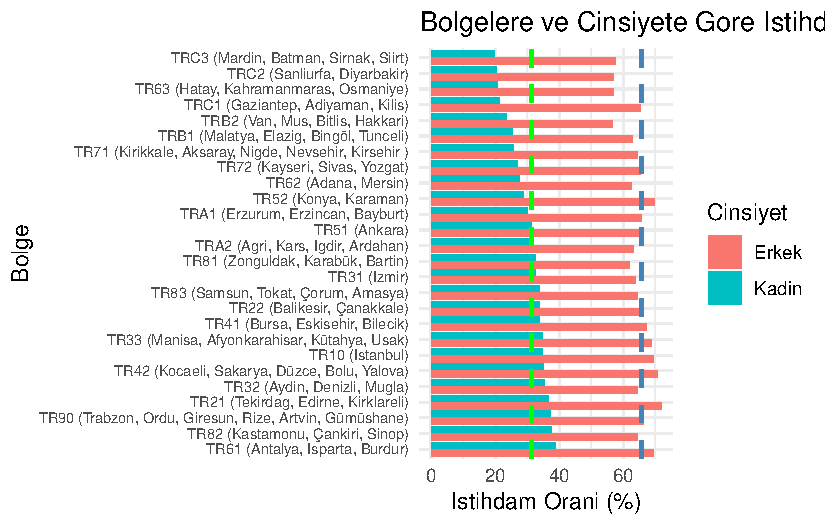
\includegraphics{project_files/figure-pdf/unnamed-chunk-3-1.pdf}

\subsection{Eğitim Durumuna Göre Yıllık Kazanç
Durumu}\label{eux11fitim-durumuna-guxf6re-yux131llux131k-kazanuxe7-durumu}

Eğitim düzeyine göre kadın ve erkek için yıllık kazanç miktarları
grafiğine bakıldığında 2023 yılı verilerine göre kazanç düzeylerinin hem
erkeklerde hem de kadınlarda eğitim durumu ile birlikte yükseldiği
görülmektedir. Ancak eğitim seviyesi arttıkça cinsiyetler arası kazanç
farkı belirginleşmektedir. Bu durum, özellikle yükseköğretim mezunları
arasında ciddi bir gelir eşitsizliğine işaret etmektedir. Eğitim
durumuna göre en yüksek yıllık ortalama brüt kazancı yükseköğretim
eğitim düzeyine sahip olanlar elde etmiş olup, bu eğitim düzeyinde
yıllık ortalama brüt kazanç erkeklerde 431 bin 364 TL, kadınlarda ise
354 bin 149 TL olmuştur. Tüm seviyelerde erkek ve kadın aynı eğitim
düzeyinde olmasına rağmen erkeklerin yıllık ortalama brüt kazancının
kadınlardan fazla olduğu görülmektedir.

\begin{Shaded}
\begin{Highlighting}[]
\FunctionTok{library}\NormalTok{(readxl)}
\FunctionTok{library}\NormalTok{(ggplot2)}
\FunctionTok{library}\NormalTok{(tidyr)}
\FunctionTok{library}\NormalTok{(dplyr)}
\FunctionTok{library}\NormalTok{(readr)}

\CommentTok{\# Geçici bir ortam oluştur ve .RData dosyasını yükle}
\NormalTok{temp\_env }\OtherTok{\textless{}{-}} \FunctionTok{new.env}\NormalTok{()}
\FunctionTok{load}\NormalTok{(}\StringTok{"kadın\_projesi\_verisi.RData"}\NormalTok{, }\AttributeTok{envir =}\NormalTok{ temp\_env)}

\CommentTok{\# Sadece yillik\_kazanc verisini al}
\NormalTok{veri }\OtherTok{\textless{}{-}}\NormalTok{ temp\_env}\SpecialCharTok{$}\NormalTok{yillik\_kazanc}

\CommentTok{\# Sütun adlarını ASCII karakterlerine dönüştür}
\FunctionTok{names}\NormalTok{(veri) }\OtherTok{\textless{}{-}} \FunctionTok{iconv}\NormalTok{(}\FunctionTok{names}\NormalTok{(veri), }\AttributeTok{from =} \StringTok{""}\NormalTok{, }\AttributeTok{to =} \StringTok{"ASCII//TRANSLIT"}\NormalTok{)}

\CommentTok{\# Grafik oluştur}
\FunctionTok{ggplot}\NormalTok{(veri, }\FunctionTok{aes}\NormalTok{(}\AttributeTok{x =} \FunctionTok{reorder}\NormalTok{(egitim\_duzeyi, yillik\_ort\_brut\_kazanc), }
                 \AttributeTok{y =}\NormalTok{ yillik\_ort\_brut\_kazanc, }\AttributeTok{fill =}\NormalTok{ cinsiyet)) }\SpecialCharTok{+}
  \FunctionTok{geom\_bar}\NormalTok{(}\AttributeTok{stat =} \StringTok{"identity"}\NormalTok{, }\AttributeTok{position =} \StringTok{"dodge"}\NormalTok{) }\SpecialCharTok{+}
  \FunctionTok{geom\_text}\NormalTok{(}\FunctionTok{aes}\NormalTok{(}\AttributeTok{label =} \FunctionTok{paste0}\NormalTok{(}\FunctionTok{format}\NormalTok{(yillik\_ort\_brut\_kazanc, }\AttributeTok{big.mark =} \StringTok{"."}\NormalTok{, }\AttributeTok{decimal.mark =} \StringTok{","}\NormalTok{), }\StringTok{",00"}\NormalTok{)), }
            \AttributeTok{position =} \FunctionTok{position\_dodge}\NormalTok{(}\AttributeTok{width =} \FloatTok{0.9}\NormalTok{), }\AttributeTok{vjust =} \SpecialCharTok{{-}}\FloatTok{0.3}\NormalTok{, }\AttributeTok{size =} \DecValTok{3}\NormalTok{) }\SpecialCharTok{+} 
  \FunctionTok{scale\_y\_continuous}\NormalTok{(}\AttributeTok{labels =}\NormalTok{ scales}\SpecialCharTok{::}\FunctionTok{comma\_format}\NormalTok{(}\AttributeTok{big.mark =} \StringTok{"."}\NormalTok{, }\AttributeTok{decimal.mark =} \StringTok{","}\NormalTok{)) }\SpecialCharTok{+}
  \FunctionTok{labs}\NormalTok{(}\AttributeTok{title =} \StringTok{"Egitim Duzeyine Gore Yillik Ortalama Brut Kazanc"}\NormalTok{,}
       \AttributeTok{x =} \StringTok{"Egitim Duzeyi"}\NormalTok{, }\AttributeTok{y =} \StringTok{"Yillik Kazanc (TL)"}\NormalTok{, }\AttributeTok{fill =} \StringTok{"Cinsiyet"}\NormalTok{) }\SpecialCharTok{+}
  \FunctionTok{theme\_minimal}\NormalTok{()}
\end{Highlighting}
\end{Shaded}

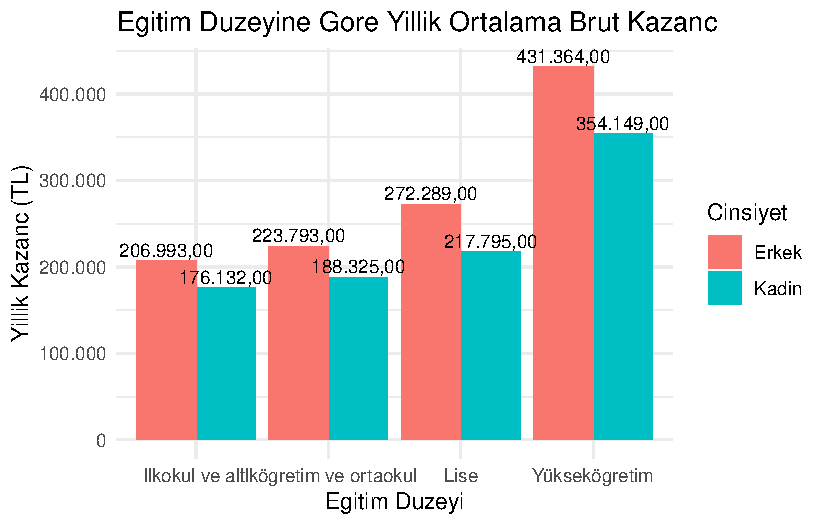
\includegraphics{project_files/figure-pdf/unnamed-chunk-4-1.pdf}

\subsection{Meslek Gruplarına Göre Kazanç
Durumu}\label{meslek-gruplarux131na-guxf6re-kazanuxe7-durumu}

Meslek gruplarına göre kadın ve erkek için yıllık ortalama kazanç
verilerinden elde edilen grafik gösterilmektedir. 2023 yılı verilerine
göre, kadınlarda en yüksek yıllık ortalama brüt kazancı 530.663,00 TL
ile yöneticiler meslek grubunda çalışanlar elde etmiştir. Yönetici
pozisyonunda çalışan erkek ve kadınlar arasında yıllık ortalama
kazançlarında farklılığın düşük olduğu dikkat çekmektedir. En düşük
yıllık ortalama brüt kazanç ise 185.860,00 TL ile nitelikli tarım,
ormancılık ve su ürünleri çalışanları grubunda gerçekleşmiştir. Yalnızca
``Hizmet ve servis elemanları'' meslek grubunda çalışan kadınlar aynı
meslek grubunda çalışan erkeklere göre daha fazla yıllık ortalama kazanç
elde etmiş, diğer tüm meslek gruplarında erkekler kadınlardan daha fazla
yıllık ortalama kazanç sağlamıştır.

\begin{Shaded}
\begin{Highlighting}[]
\FunctionTok{library}\NormalTok{(readxl)}
\FunctionTok{library}\NormalTok{(ggplot2)}
\FunctionTok{library}\NormalTok{(tidyr)}
\FunctionTok{library}\NormalTok{(dplyr)}
\FunctionTok{library}\NormalTok{(readr)}
\FunctionTok{library}\NormalTok{(scales)}


\CommentTok{\# Geçici bir ortam oluştur ve RData dosyasını yükle}
\NormalTok{temp\_env }\OtherTok{\textless{}{-}} \FunctionTok{new.env}\NormalTok{()}
\FunctionTok{load}\NormalTok{(}\StringTok{"kadın\_projesi\_verisi.RData"}\NormalTok{, }\AttributeTok{envir =}\NormalTok{ temp\_env)}

\CommentTok{\# İlgili veri setini al}
\NormalTok{veri }\OtherTok{\textless{}{-}}\NormalTok{ temp\_env}\SpecialCharTok{$}\NormalTok{meslek\_gruplarina\_gore\_kazanc}


\CommentTok{\# Veriyi meslek ve cinsiyete göre sıralayın}
\NormalTok{veri }\OtherTok{\textless{}{-}}\NormalTok{ veri }\SpecialCharTok{\%\textgreater{}\%}
  \FunctionTok{group\_by}\NormalTok{(meslek, cinsiyet) }\SpecialCharTok{\%\textgreater{}\%}
  \FunctionTok{summarize}\NormalTok{(}\AttributeTok{yillik\_ort\_kazanc =} \FunctionTok{mean}\NormalTok{(yillik\_ort\_kazanc, }\AttributeTok{na.rm =} \ConstantTok{TRUE}\NormalTok{, }\AttributeTok{.groups =} \StringTok{"drop"}\NormalTok{))}

\CommentTok{\# Kadınlara göre meslek sıralaması}
\NormalTok{sirali\_meslekler }\OtherTok{\textless{}{-}}\NormalTok{ veri }\SpecialCharTok{\%\textgreater{}\%}
  \FunctionTok{filter}\NormalTok{(cinsiyet }\SpecialCharTok{==} \StringTok{"Kadın"}\NormalTok{) }\SpecialCharTok{\%\textgreater{}\%}
  \FunctionTok{arrange}\NormalTok{(yillik\_ort\_kazanc) }\SpecialCharTok{\%\textgreater{}\%}
  \FunctionTok{pull}\NormalTok{(meslek)}

\CommentTok{\# Sıralı faktör olarak ayarla}
\NormalTok{veri}\SpecialCharTok{$}\NormalTok{meslek }\OtherTok{\textless{}{-}} \FunctionTok{factor}\NormalTok{(veri}\SpecialCharTok{$}\NormalTok{meslek, }\AttributeTok{levels =}\NormalTok{ sirali\_meslekler)}

\CommentTok{\# Grafik oluşturma}
\FunctionTok{ggplot}\NormalTok{(veri, }\FunctionTok{aes}\NormalTok{(}\AttributeTok{x =}\NormalTok{ meslek, }\AttributeTok{y =}\NormalTok{ yillik\_ort\_kazanc, }\AttributeTok{fill =}\NormalTok{ cinsiyet)) }\SpecialCharTok{+}
  \FunctionTok{geom\_bar}\NormalTok{(}\AttributeTok{stat =} \StringTok{"identity"}\NormalTok{, }\AttributeTok{position =} \StringTok{"dodge"}\NormalTok{) }\SpecialCharTok{+}
  \FunctionTok{geom\_text}\NormalTok{(}\FunctionTok{aes}\NormalTok{(}\AttributeTok{label =} \FunctionTok{format}\NormalTok{(yillik\_ort\_kazanc, }\AttributeTok{big.mark =} \StringTok{"."}\NormalTok{, }\AttributeTok{decimal.mark =} \StringTok{","}\NormalTok{, }\AttributeTok{nsmall =} \DecValTok{2}\NormalTok{)),}
            \AttributeTok{position =} \FunctionTok{position\_dodge}\NormalTok{(}\AttributeTok{width =} \FloatTok{0.9}\NormalTok{), }
            \AttributeTok{hjust =} \SpecialCharTok{{-}}\FloatTok{0.1}\NormalTok{, }\AttributeTok{size =} \FloatTok{2.5}\NormalTok{) }\SpecialCharTok{+}  \CommentTok{\# ← etiketler çubuğun sağında}
  \FunctionTok{coord\_flip}\NormalTok{() }\SpecialCharTok{+}
  \FunctionTok{scale\_fill\_manual}\NormalTok{(}\AttributeTok{values =} \FunctionTok{c}\NormalTok{(}\StringTok{"Kadın"} \OtherTok{=} \StringTok{"yellow"}\NormalTok{, }\StringTok{"Erkek"} \OtherTok{=} \StringTok{"lightgreen"}\NormalTok{)) }\SpecialCharTok{+}
  \FunctionTok{scale\_y\_continuous}\NormalTok{(}
    \AttributeTok{breaks =} \FunctionTok{c}\NormalTok{(}\DecValTok{0}\NormalTok{, }\DecValTok{100000}\NormalTok{, }\DecValTok{300000}\NormalTok{, }\DecValTok{500000}\NormalTok{),}
    \AttributeTok{labels =} \FunctionTok{label\_number}\NormalTok{(}\AttributeTok{big.mark =} \StringTok{"."}\NormalTok{, }\AttributeTok{decimal.mark =} \StringTok{","}\NormalTok{, }\AttributeTok{accuracy =} \DecValTok{1}\NormalTok{),}
    \AttributeTok{expand =} \FunctionTok{expansion}\NormalTok{(}\AttributeTok{mult =} \FunctionTok{c}\NormalTok{(}\DecValTok{0}\NormalTok{, }\FloatTok{0.25}\NormalTok{))  }\CommentTok{\# ← boşluk bırak, çubukların sonunda etiketler için alan yarat}
\NormalTok{  ) }\SpecialCharTok{+}
  \FunctionTok{labs}\NormalTok{(}\AttributeTok{title =} \StringTok{"Ortalama Kazanc"}\NormalTok{,}
       \AttributeTok{x =} \StringTok{"Meslek Grubu"}\NormalTok{, }\AttributeTok{y =} \StringTok{"Yillik Ortalama Kazanc (TL)"}\NormalTok{, }\AttributeTok{fill =} \StringTok{"Cinsiyet"}\NormalTok{) }\SpecialCharTok{+}
  \FunctionTok{theme\_minimal}\NormalTok{() }\SpecialCharTok{+}
  \FunctionTok{theme}\NormalTok{(}\AttributeTok{axis.text.y =} \FunctionTok{element\_text}\NormalTok{(}\AttributeTok{margin =} \FunctionTok{margin}\NormalTok{(}\AttributeTok{r =} \DecValTok{10}\NormalTok{)))}
\end{Highlighting}
\end{Shaded}

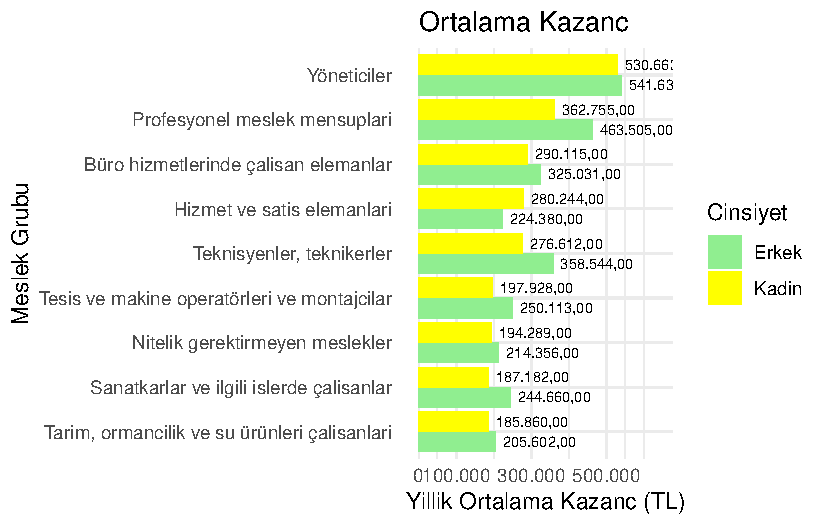
\includegraphics{project_files/figure-pdf/unnamed-chunk-5-1.pdf}

\subsection{Üst ve Orta Düzey Yönetici Pozisyonundaki
Görünüm}\label{uxfcst-ve-orta-duxfczey-yuxf6netici-pozisyonundaki-guxf6ruxfcnuxfcm}

Yıllara göre kadın ve erkek için üst ve orta düzey yönetici olma oranı
grafikte gösterilmektedir. Üst ve orta düzey yönetici pozisyonundaki
kadın oranı 2015 yılında \%14.4 iken 2023 yılında \%20.6 olmuştur. Bu
artış, kadınların liderlik pozisyonlarında görünürlüğünün zamanla
arttığını göstermektedir. Ancak artış hızı yavaş ve sınırlı kalmıştır.
Bu oran erkeklerde 2015 yılında \%85.5 iken 2023 yılında \%79.4 olarak
gerçekleşmiştir. Bu düşüş, kadınların yönetime daha fazla dâhil olmaya
başladığını gösterse de, erkekler hâlâ yönetici pozisyonlarının büyük
çoğunluğunu elinde bulundurmaktadır. 2015-2023 yıllarındaki orta ve üst
düzey yönetici oranları incelendiğinde tüm yıllarda kadınların yönetici
pozisyonunda erkeklerle kıyaslandığında çok daha az yer bulabildiği
görülmektedir.

\begin{Shaded}
\begin{Highlighting}[]
\FunctionTok{library}\NormalTok{(readxl)}
\FunctionTok{library}\NormalTok{(ggplot2)}
\FunctionTok{library}\NormalTok{(tidyr)}
\FunctionTok{library}\NormalTok{(dplyr)}
\FunctionTok{library}\NormalTok{(readr)}

\CommentTok{\# Geçici ortam oluştur ve .RData dosyasını yükle}
\NormalTok{temp\_env }\OtherTok{\textless{}{-}} \FunctionTok{new.env}\NormalTok{()}
\FunctionTok{load}\NormalTok{(}\StringTok{"kadın\_projesi\_verisi.RData"}\NormalTok{, }\AttributeTok{envir =}\NormalTok{ temp\_env)}

\CommentTok{\# Sadece \textquotesingle{}yonetici\textquotesingle{} verisini al}
\NormalTok{veri }\OtherTok{\textless{}{-}}\NormalTok{ temp\_env}\SpecialCharTok{$}\NormalTok{yonetici}

\CommentTok{\# Sütun adlarını ASCII formatına çevir (Türkçe karakter hatası önlemi)}
\FunctionTok{names}\NormalTok{(veri) }\OtherTok{\textless{}{-}} \FunctionTok{iconv}\NormalTok{(}\FunctionTok{names}\NormalTok{(veri), }\AttributeTok{from =} \StringTok{""}\NormalTok{, }\AttributeTok{to =} \StringTok{"ASCII//TRANSLIT"}\NormalTok{)}

\CommentTok{\# Veriyi düzenle}
\NormalTok{veri }\OtherTok{\textless{}{-}}\NormalTok{ veri }\SpecialCharTok{\%\textgreater{}\%}
  \FunctionTok{mutate}\NormalTok{(}
    \AttributeTok{cinsiyet =} \FunctionTok{as.character}\NormalTok{(cinsiyet),}
    \AttributeTok{orta\_ust\_yonetici\_orani =} \FunctionTok{as.numeric}\NormalTok{(orta\_ust\_yonetici\_orani)}
\NormalTok{  ) }\SpecialCharTok{\%\textgreater{}\%}
  \FunctionTok{filter}\NormalTok{(cinsiyet }\SpecialCharTok{\%in\%} \FunctionTok{c}\NormalTok{(}\StringTok{"Kadın"}\NormalTok{, }\StringTok{"Erkek"}\NormalTok{)) }\SpecialCharTok{\%\textgreater{}\%}
  \FunctionTok{mutate}\NormalTok{(}\AttributeTok{cinsiyet =} \FunctionTok{factor}\NormalTok{(cinsiyet, }\AttributeTok{levels =} \FunctionTok{c}\NormalTok{(}\StringTok{"Kadın"}\NormalTok{, }\StringTok{"Erkek"}\NormalTok{)))}

\CommentTok{\# Grafik oluştur}
\FunctionTok{ggplot}\NormalTok{(veri, }\FunctionTok{aes}\NormalTok{(}\AttributeTok{x =} \FunctionTok{as.factor}\NormalTok{(yil), }\AttributeTok{y =}\NormalTok{ orta\_ust\_yonetici\_orani, }\AttributeTok{color =}\NormalTok{ cinsiyet, }\AttributeTok{group =}\NormalTok{ cinsiyet)) }\SpecialCharTok{+}
  \FunctionTok{geom\_line}\NormalTok{(}\AttributeTok{linewidth =} \DecValTok{1}\NormalTok{) }\SpecialCharTok{+}
  \FunctionTok{geom\_point}\NormalTok{(}\AttributeTok{size =} \DecValTok{2}\NormalTok{) }\SpecialCharTok{+}
  \FunctionTok{geom\_text}\NormalTok{(}
    \FunctionTok{aes}\NormalTok{(}\AttributeTok{label =} \FunctionTok{sprintf}\NormalTok{(}\StringTok{"\%.1f"}\NormalTok{, orta\_ust\_yonetici\_orani)),}
    \AttributeTok{vjust =} \SpecialCharTok{{-}}\FloatTok{0.5}\NormalTok{,}
    \AttributeTok{size =} \DecValTok{3}\NormalTok{,}
    \AttributeTok{show.legend =} \ConstantTok{FALSE}
\NormalTok{  ) }\SpecialCharTok{+}
  \FunctionTok{labs}\NormalTok{(}\AttributeTok{title =} \StringTok{"Yillara Gore Orta ve Ust Duzey Yonetici Olma Orani"}\NormalTok{,}
       \AttributeTok{x =} \StringTok{"Yil"}\NormalTok{,}
       \AttributeTok{y =} \StringTok{"Orta ve Ust Duzey Yonetici Orani (\%)"}\NormalTok{,}
       \AttributeTok{color =} \StringTok{"Cinsiyet"}\NormalTok{) }\SpecialCharTok{+}
  \FunctionTok{scale\_color\_manual}\NormalTok{(}\AttributeTok{values =} \FunctionTok{c}\NormalTok{(}\StringTok{"Kadın"} \OtherTok{=} \StringTok{"purple"}\NormalTok{, }\StringTok{"Erkek"} \OtherTok{=} \StringTok{"orange"}\NormalTok{)) }\SpecialCharTok{+}
  \FunctionTok{theme\_minimal}\NormalTok{()}
\end{Highlighting}
\end{Shaded}

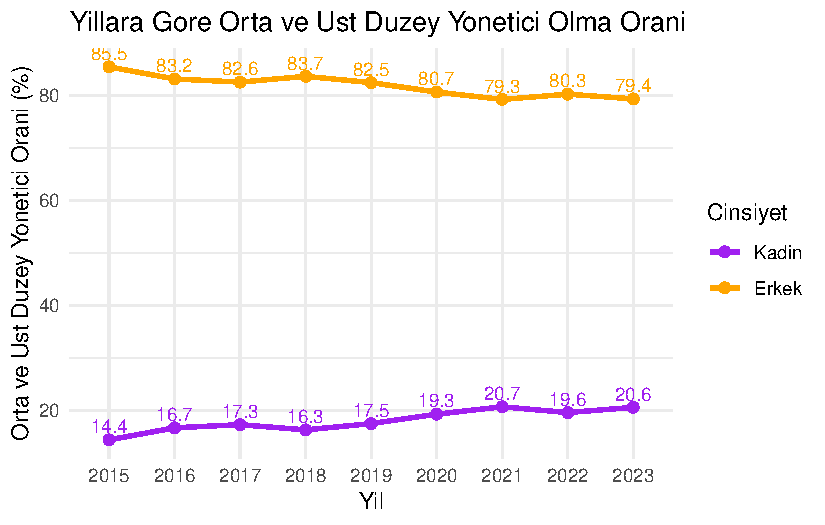
\includegraphics{project_files/figure-pdf/unnamed-chunk-6-1.pdf}

\subsection{Çocuğa Bağlı İstihdam
Oranı}\label{uxe7ocuux11fa-baux11flux131-istihdam-oranux131}

Üç yaş altı çocuk sahibi olma durumuna göre kadın ve erkek için yıllara
göre istihdam oranları grafikte gösterilmektedir. 2023 yılında hanesinde
3 yaşın altında çocuğu olan 25-49 yaş grubundaki kadınların istihdam
oranının \%27,1, erkeklerin istihdam oranının ise \%90,6 olduğu
görülmüştür. 2023 yılında çocuk sahibi olmayan kadınların istihdam oranı
\%58 iken, erkekler için bu oran \%79.3'tür.

2015-2023 yılları için veriler incelendiğinde çocuk sahibi olmayan
kadınların istihdam oranının, 3 yaş altı çocuk sahibi olan kadınlara
kıyasla tüm yıllar için neredeyse iki katı olduğu görülmektedir. Bu
durum erkeklerde ters etki yaratmaktadır. 3 yaş altı çocuk sahibi olan
erkeklerin istihdam oranı, çocuk sahibi olmayanlara göre daha fazladır.
Bu grafik, bakım yükümlülüklerinin cinsiyetler arasında eşit
dağılmadığını açıkça göstermektedir. Erkeklerin çocuk sahibi olduktan
sonra istihdam oranları büyük ölçüde korunurken, kadınların istihdam
oranı keskin şekilde düşmektedir.

\begin{Shaded}
\begin{Highlighting}[]
\FunctionTok{library}\NormalTok{(readxl)}
\FunctionTok{library}\NormalTok{(ggplot2)}
\FunctionTok{library}\NormalTok{(tidyr)}
\FunctionTok{library}\NormalTok{(dplyr)}
\FunctionTok{library}\NormalTok{(readr)}

\CommentTok{\# Geçici bir ortam oluştur ve .RData dosyasını yükle}
\NormalTok{temp\_env }\OtherTok{\textless{}{-}} \FunctionTok{new.env}\NormalTok{()}
\FunctionTok{load}\NormalTok{(}\StringTok{"kadın\_projesi\_verisi.RData"}\NormalTok{, }\AttributeTok{envir =}\NormalTok{ temp\_env)}

\CommentTok{\# Veriyi çağır}
\NormalTok{veri }\OtherTok{\textless{}{-}}\NormalTok{ temp\_env}\SpecialCharTok{$}\NormalTok{cocuga\_bagli\_istihdam\_orani}

\CommentTok{\# Uzun formata dönüştür (pivot\_longer)}
\NormalTok{veri\_long }\OtherTok{\textless{}{-}}\NormalTok{ veri }\SpecialCharTok{\%\textgreater{}\%}
  \FunctionTok{pivot\_longer}\NormalTok{(}
    \AttributeTok{cols =} \FunctionTok{c}\NormalTok{(}\StringTok{"3yasalti\_cocuk\_olan\_istihdam\_orani"}\NormalTok{, }\StringTok{"cocuk\_olmayan\_istihdam\_orani"}\NormalTok{), }
    \AttributeTok{names\_to =} \StringTok{"cocuk\_durumu"}\NormalTok{, }
    \AttributeTok{values\_to =} \StringTok{"istihdam\_orani"}
\NormalTok{  ) }\SpecialCharTok{\%\textgreater{}\%}
  \FunctionTok{mutate}\NormalTok{(}\AttributeTok{cocuk\_durumu =} \FunctionTok{recode}\NormalTok{(cocuk\_durumu, }
    \StringTok{"3yasalti\_cocuk\_olan\_istihdam\_orani"} \OtherTok{=} \StringTok{"3 Yaş Altı Çocuk Sahibi"}\NormalTok{,}
    \StringTok{"cocuk\_olmayan\_istihdam\_orani"} \OtherTok{=} \StringTok{"Çocuk Sahibi Değil"}
\NormalTok{  ))}

\CommentTok{\# Grafik oluştur}
\FunctionTok{ggplot}\NormalTok{(veri\_long, }\FunctionTok{aes}\NormalTok{(}\AttributeTok{x =} \FunctionTok{as.factor}\NormalTok{(yil), }\AttributeTok{y =}\NormalTok{ istihdam\_orani, }\AttributeTok{color =}\NormalTok{ cinsiyet, }
                      \AttributeTok{linetype =}\NormalTok{ cocuk\_durumu, }\AttributeTok{group =} \FunctionTok{interaction}\NormalTok{(cinsiyet, cocuk\_durumu))) }\SpecialCharTok{+}
  \FunctionTok{geom\_line}\NormalTok{(}\AttributeTok{linewidth =} \FloatTok{1.2}\NormalTok{) }\SpecialCharTok{+}
  \FunctionTok{geom\_point}\NormalTok{(}\AttributeTok{size =} \DecValTok{3}\NormalTok{) }\SpecialCharTok{+}
  \FunctionTok{geom\_text}\NormalTok{(}\FunctionTok{aes}\NormalTok{(}\AttributeTok{label =} \FunctionTok{round}\NormalTok{(istihdam\_orani, }\DecValTok{1}\NormalTok{)), }
            \AttributeTok{vjust =} \SpecialCharTok{{-}}\FloatTok{0.9}\NormalTok{, }\AttributeTok{size =} \DecValTok{3}\NormalTok{, }\AttributeTok{show.legend =} \ConstantTok{FALSE}\NormalTok{) }\SpecialCharTok{+}
  \FunctionTok{labs}\NormalTok{(}\AttributeTok{title =} \StringTok{"Yillara Gore 3 Yas Alti Cocuk Sahibi Olma Durumuna Gore Istihdam Orani"}\NormalTok{,}
       \AttributeTok{x =} \StringTok{"Yil"}\NormalTok{,}
       \AttributeTok{y =} \StringTok{"Istihdam Orani (\%)"}\NormalTok{,}
       \AttributeTok{color =} \StringTok{"Cinsiyet"}\NormalTok{,}
       \AttributeTok{linetype =} \StringTok{"Cocuk Durumu"}\NormalTok{) }\SpecialCharTok{+}
  \FunctionTok{scale\_x\_discrete}\NormalTok{(}\AttributeTok{breaks =} \FunctionTok{unique}\NormalTok{(veri\_long}\SpecialCharTok{$}\NormalTok{yil)) }\SpecialCharTok{+}
  \FunctionTok{scale\_y\_continuous}\NormalTok{(}\AttributeTok{breaks =} \FunctionTok{seq}\NormalTok{(}\DecValTok{0}\NormalTok{, }\DecValTok{90}\NormalTok{, }\AttributeTok{by =} \DecValTok{10}\NormalTok{)) }\SpecialCharTok{+}
  \FunctionTok{theme\_minimal}\NormalTok{() }\SpecialCharTok{+}
  \FunctionTok{scale\_color\_manual}\NormalTok{(}\AttributeTok{values =} \FunctionTok{c}\NormalTok{(}\StringTok{"royalblue"}\NormalTok{, }\StringTok{"hotpink"}\NormalTok{))}
\end{Highlighting}
\end{Shaded}

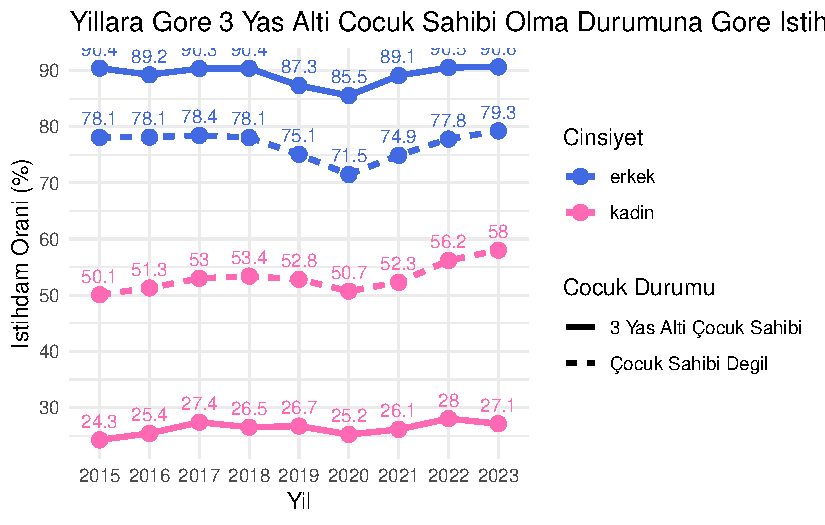
\includegraphics{project_files/figure-pdf/unnamed-chunk-7-1.pdf}

\subsection{Analiz}\label{analiz-1}

işgücü verileri kullanılarak iki temel model oluşturulmuştur: İstihdam
Oranı Modeli ve İşsizlik Oranı Modeli.

Analizde, cinsiyet ve eğitim düzeyi arasındaki etkileşimi gözlemlemek
için doğrusal regresyon modelleri kullanılmıştır.

\subsection{İstihdam Oranı Modeli}\label{istihdam-oranux131-modeli}

İstihdam oranı, işgücünün hangi oranda ekonomik faaliyetlere
katılabildiğini göstermesi bakımından önemlidir. İstihdam edilen
kişilerin kurumsal olmayan çalışma çağındaki nüfusa oranı, istihdam
oranını ifade etmektedir. Bu modelde, istihdam oranı bağımlı değişken
olarak alınmış, eğitim düzeyi ve cinsiyet bağımsız değişken olarak
modele dahil edilmiştir. Model, eğitim düzeyi ve cinsiyet arasındaki
etkileşimi de göz önünde bulunduracak şekilde formüle edilmiştir:

İstihdam Oranı = β0 + β1 × Eğitim Düzeyi + β2 × Cinsiyet + β3 × (Eğitim
Düzeyi × Cinsiyet) + ϵ

\subsection{İşsizlik Oranı Modeli}\label{iux15fsizlik-oranux131-modeli}

İşsizlik oranı, bir ekonomide işi olmayıp iş arayanların işgücüne
oranıdır. İşsizlik oranı ekonominin performansını yansıtması bakımından
oldukça önemlidir. Bu modelde işsizlik oranı bağımlı değişken olarak
kullanılmış ve benzer şekilde eğitim düzeyi ile cinsiyet arasındaki
etkileşim dikkate alınarak analiz edilmiştir:

İşsizlik Oranı = β0 + β1 × Eğitim Düzeyi + β2 × Cinsiyet + β3 × (Eğitim
Düzeyi × Cinsiyet) + ϵ

\begin{Shaded}
\begin{Highlighting}[]
\CommentTok{\# Geçici ortam oluştur ve RData dosyasını yükle}
\NormalTok{temp\_env }\OtherTok{\textless{}{-}} \FunctionTok{new.env}\NormalTok{()}
\FunctionTok{load}\NormalTok{(}\StringTok{"kadın\_projesi\_verisi.RData"}\NormalTok{, }\AttributeTok{envir =}\NormalTok{ temp\_env)}

\CommentTok{\# Veriyi al}
\NormalTok{veri }\OtherTok{\textless{}{-}}\NormalTok{ temp\_env}\SpecialCharTok{$}\NormalTok{isgucu\_verisi}

\CommentTok{\# Eksik verileri grup ortalaması ile doldur}
\NormalTok{veri }\OtherTok{\textless{}{-}}\NormalTok{ veri }\SpecialCharTok{\%\textgreater{}\%}
  \FunctionTok{group\_by}\NormalTok{(cinsiyet, egitim\_duzeyi) }\SpecialCharTok{\%\textgreater{}\%}
  \FunctionTok{mutate}\NormalTok{(}
    \AttributeTok{issizlik\_orani =} \FunctionTok{ifelse}\NormalTok{(}\FunctionTok{is.na}\NormalTok{(issizlik\_orani), }\FunctionTok{mean}\NormalTok{(issizlik\_orani, }\AttributeTok{na.rm =} \ConstantTok{TRUE}\NormalTok{), issizlik\_orani),}
    \AttributeTok{istihdam\_orani =} \FunctionTok{ifelse}\NormalTok{(}\FunctionTok{is.na}\NormalTok{(istihdam\_orani), }\FunctionTok{mean}\NormalTok{(istihdam\_orani, }\AttributeTok{na.rm =} \ConstantTok{TRUE}\NormalTok{), istihdam\_orani)}
\NormalTok{  ) }\SpecialCharTok{\%\textgreater{}\%}
  \FunctionTok{ungroup}\NormalTok{()}

\CommentTok{\# Eğitim düzeyine sıralama ekle}
\NormalTok{veri }\OtherTok{\textless{}{-}}\NormalTok{ veri }\SpecialCharTok{\%\textgreater{}\%}
  \FunctionTok{mutate}\NormalTok{(}\AttributeTok{egitim\_sira =} \FunctionTok{case\_when}\NormalTok{(}
\NormalTok{    egitim\_duzeyi }\SpecialCharTok{==} \StringTok{"Okuma yazma bilmeyen"} \SpecialCharTok{\textasciitilde{}} \DecValTok{1}\NormalTok{,}
\NormalTok{    egitim\_duzeyi }\SpecialCharTok{==} \StringTok{"Ilkogretim"} \SpecialCharTok{\textasciitilde{}} \DecValTok{2}\NormalTok{,}
\NormalTok{    egitim\_duzeyi }\SpecialCharTok{==} \StringTok{"Genel lise"} \SpecialCharTok{\textasciitilde{}} \DecValTok{3}\NormalTok{,}
\NormalTok{    egitim\_duzeyi }\SpecialCharTok{==} \StringTok{"Lise dengi mesleki okul"} \SpecialCharTok{\textasciitilde{}} \DecValTok{4}\NormalTok{,}
\NormalTok{    egitim\_duzeyi }\SpecialCharTok{==} \StringTok{"Yuksekogretim"} \SpecialCharTok{\textasciitilde{}} \DecValTok{5}\NormalTok{,}
    \ConstantTok{TRUE} \SpecialCharTok{\textasciitilde{}} \ConstantTok{NA\_real\_}
\NormalTok{  ))}

\CommentTok{\# Cinsiyeti faktöre çevir}
\NormalTok{veri}\SpecialCharTok{$}\NormalTok{cinsiyet }\OtherTok{\textless{}{-}} \FunctionTok{factor}\NormalTok{(veri}\SpecialCharTok{$}\NormalTok{cinsiyet)}

\CommentTok{\# Regresyon modelleri}
\NormalTok{model\_istihdam }\OtherTok{\textless{}{-}} \FunctionTok{lm}\NormalTok{(istihdam\_orani }\SpecialCharTok{\textasciitilde{}}\NormalTok{ egitim\_sira }\SpecialCharTok{*}\NormalTok{ cinsiyet, }\AttributeTok{data =}\NormalTok{ veri)}
\NormalTok{model\_issizlik }\OtherTok{\textless{}{-}} \FunctionTok{lm}\NormalTok{(issizlik\_orani }\SpecialCharTok{\textasciitilde{}}\NormalTok{ egitim\_sira }\SpecialCharTok{*}\NormalTok{ cinsiyet, }\AttributeTok{data =}\NormalTok{ veri)}

\FunctionTok{summary}\NormalTok{(model\_istihdam)}
\end{Highlighting}
\end{Shaded}

\begin{verbatim}

Call:
lm(formula = istihdam_orani ~ egitim_sira * cinsiyet, data = veri)

Residuals:
     Min       1Q   Median       3Q      Max 
-17.3513  -6.2798  -0.5857   4.2327  22.2960 

Coefficients:
                          Estimate Std. Error t value Pr(>|t|)    
(Intercept)                39.7987     2.7273  14.593  < 2e-16 ***
egitim_sira                 9.0527     0.8223  11.009  < 2e-16 ***
cinsiyetKadın             -31.4200     3.8570  -8.146 1.39e-12 ***
egitim_sira:cinsiyetKadın  -0.5140     1.1629  -0.442    0.659    
---
Signif. codes:  0 '***' 0.001 '**' 0.01 '*' 0.05 '.' 0.1 ' ' 1

Residual standard error: 8.223 on 96 degrees of freedom
Multiple R-squared:  0.8679,    Adjusted R-squared:  0.8638 
F-statistic: 210.2 on 3 and 96 DF,  p-value: < 2.2e-16
\end{verbatim}

\begin{Shaded}
\begin{Highlighting}[]
\FunctionTok{summary}\NormalTok{(model\_issizlik)}
\end{Highlighting}
\end{Shaded}

\begin{verbatim}

Call:
lm(formula = issizlik_orani ~ egitim_sira * cinsiyet, data = veri)

Residuals:
   Min     1Q Median     3Q    Max 
-7.974 -2.178  0.311  2.336  7.390 

Coefficients:
                          Estimate Std. Error t value Pr(>|t|)    
(Intercept)                16.7780     1.2305  13.635  < 2e-16 ***
egitim_sira                -1.7540     0.3710  -4.728 7.78e-06 ***
cinsiyetKadın              -9.0240     1.7401  -5.186 1.19e-06 ***
egitim_sira:cinsiyetKadın   4.4180     0.5247   8.420 3.63e-13 ***
---
Signif. codes:  0 '***' 0.001 '**' 0.01 '*' 0.05 '.' 0.1 ' ' 1

Residual standard error: 3.71 on 96 degrees of freedom
Multiple R-squared:  0.5257,    Adjusted R-squared:  0.5109 
F-statistic: 35.47 on 3 and 96 DF,  p-value: 1.624e-15
\end{verbatim}

\begin{Shaded}
\begin{Highlighting}[]
\CommentTok{\# Grafik tema ve renk ayarları}
\NormalTok{my\_colors }\OtherTok{\textless{}{-}} \FunctionTok{c}\NormalTok{(}\StringTok{"Kadın"} \OtherTok{=} \StringTok{"darkred"}\NormalTok{, }\StringTok{"Erkek"} \OtherTok{=} \StringTok{"steelblue"}\NormalTok{)}
\NormalTok{my\_theme }\OtherTok{\textless{}{-}} \FunctionTok{theme\_minimal}\NormalTok{(}\AttributeTok{base\_size =} \DecValTok{12}\NormalTok{)}

\CommentTok{\# Grafik 1: İstihdam Oranı}
\NormalTok{g1 }\OtherTok{\textless{}{-}} \FunctionTok{ggplot}\NormalTok{(veri, }\FunctionTok{aes}\NormalTok{(}\AttributeTok{x =}\NormalTok{ egitim\_sira, }\AttributeTok{y =}\NormalTok{ istihdam\_orani, }\AttributeTok{color =}\NormalTok{ cinsiyet)) }\SpecialCharTok{+}
  \FunctionTok{geom\_point}\NormalTok{(}\AttributeTok{size =} \DecValTok{1}\NormalTok{) }\SpecialCharTok{+}
  \FunctionTok{geom\_smooth}\NormalTok{(}\AttributeTok{method =} \StringTok{"lm"}\NormalTok{, }\AttributeTok{se =} \ConstantTok{FALSE}\NormalTok{, }\AttributeTok{linewidth =} \FloatTok{1.2}\NormalTok{) }\SpecialCharTok{+}
  \FunctionTok{scale\_color\_manual}\NormalTok{(}\AttributeTok{values =}\NormalTok{ my\_colors) }\SpecialCharTok{+}
  \FunctionTok{scale\_x\_continuous}\NormalTok{(}
    \AttributeTok{breaks =} \DecValTok{1}\SpecialCharTok{:}\DecValTok{5}\NormalTok{,}
    \AttributeTok{labels =} \FunctionTok{c}\NormalTok{(}\StringTok{"Okuma Yazma Bilmeyen"}\NormalTok{, }\StringTok{"Ilkogretim"}\NormalTok{, }\StringTok{"Genel Lise"}\NormalTok{, }\StringTok{"Meslek Lisesi"}\NormalTok{, }\StringTok{"Yuksekogretim"}\NormalTok{)}
\NormalTok{  ) }\SpecialCharTok{+}
  \FunctionTok{labs}\NormalTok{(}\AttributeTok{title =} \StringTok{"Egitim Duzeyine Gore Istihdam Orani"}\NormalTok{,}
       \AttributeTok{x =} \StringTok{"Egitim Duzeyi"}\NormalTok{, }\AttributeTok{y =} \StringTok{"Istihdam Orani (\%)"}\NormalTok{, }\AttributeTok{color =} \StringTok{"Cinsiyet"}\NormalTok{) }\SpecialCharTok{+}
\NormalTok{  my\_theme}

\CommentTok{\# Grafik 2: İşsizlik Oranı}
\NormalTok{g2 }\OtherTok{\textless{}{-}} \FunctionTok{ggplot}\NormalTok{(veri, }\FunctionTok{aes}\NormalTok{(}\AttributeTok{x =}\NormalTok{ egitim\_sira, }\AttributeTok{y =}\NormalTok{ issizlik\_orani, }\AttributeTok{color =}\NormalTok{ cinsiyet)) }\SpecialCharTok{+}
  \FunctionTok{geom\_point}\NormalTok{(}\AttributeTok{size =} \DecValTok{1}\NormalTok{) }\SpecialCharTok{+}
  \FunctionTok{geom\_smooth}\NormalTok{(}\AttributeTok{method =} \StringTok{"lm"}\NormalTok{, }\AttributeTok{se =} \ConstantTok{FALSE}\NormalTok{, }\AttributeTok{linewidth =} \FloatTok{1.2}\NormalTok{) }\SpecialCharTok{+}
  \FunctionTok{scale\_color\_manual}\NormalTok{(}\AttributeTok{values =}\NormalTok{ my\_colors) }\SpecialCharTok{+}
  \FunctionTok{scale\_x\_continuous}\NormalTok{(}
    \AttributeTok{breaks =} \DecValTok{1}\SpecialCharTok{:}\DecValTok{5}\NormalTok{,}
    \AttributeTok{labels =} \FunctionTok{c}\NormalTok{(}\StringTok{"Okuma Yazma Bilmeyen"}\NormalTok{, }\StringTok{"Ilkogretim"}\NormalTok{, }\StringTok{"Genel Lise"}\NormalTok{, }\StringTok{"Meslek Lisesi"}\NormalTok{, }\StringTok{"Yuksekogretim"}\NormalTok{)}
\NormalTok{  ) }\SpecialCharTok{+}
  \FunctionTok{labs}\NormalTok{(}\AttributeTok{title =} \StringTok{"Egitim Duzeyine Gore Issizlik Orani"}\NormalTok{,}
       \AttributeTok{x =} \StringTok{"Egitim Duzeyi"}\NormalTok{, }\AttributeTok{y =} \StringTok{"Issizlik Orani (\%)"}\NormalTok{, }\AttributeTok{color =} \StringTok{"Cinsiyet"}\NormalTok{) }\SpecialCharTok{+}
\NormalTok{  my\_theme}

\CommentTok{\# İki grafiği birlikte göster}
\NormalTok{g1 }\SpecialCharTok{/}\NormalTok{ g2 }\SpecialCharTok{+} \FunctionTok{plot\_layout}\NormalTok{(}\AttributeTok{ncol =} \DecValTok{1}\NormalTok{)}
\end{Highlighting}
\end{Shaded}

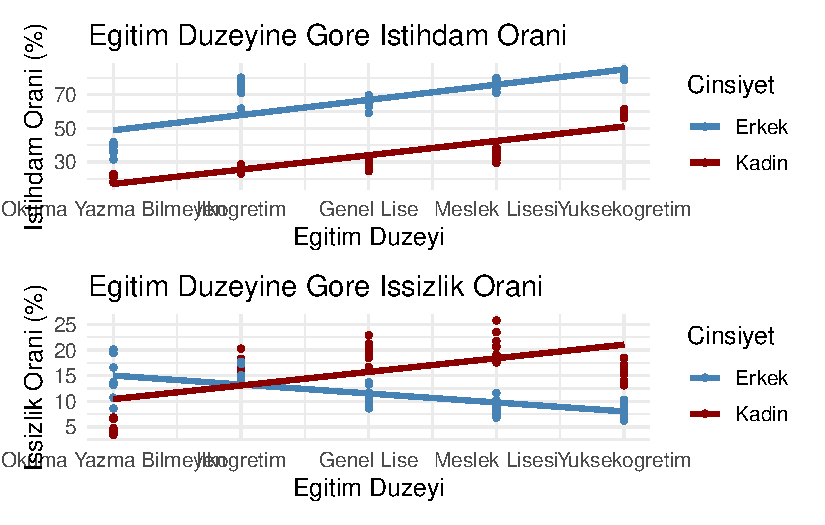
\includegraphics{project_files/figure-pdf/unnamed-chunk-8-1.pdf}

\subsection{4. Bulgular}\label{bulgular}

Bu çalışmada, eğitim düzeyi ile istihdam ve işsizlik oranları arasındaki
ilişkiler, cinsiyet farklılıkları dikkate alınarak oluşturulan iki ayrı
etkileşimli doğrusal regresyon modeli ile analiz edilmiştir. Her iki
modelde de eğitim düzeyi (egitim\_sira), cinsiyet ve bu iki değişkenin
etkileşim terimi bağımsız değişken olarak kullanılmıştır. Eğitim
düzeyine göre kadın ve erkek için istihdam oranı ve işsizlik oranı
grafiklerle sunulmuştur. Grafiklerde kullanılan eğri çizgiler, doğrusal
regresyon eğilimlerini göstermektedir.

İstihdam oranı analizine göre; Erkek bireylerde eğitim düzeyindeki her
bir artışın istihdam oranını ortalama \%9,05 oranında artırdığı
görülmektedir (p \textless{} 0.001). Cinsiyet değişkeni açısından
bakıldığında, kadın bireylerin eğitim düzeyi sabit tutulduğunda,
istihdam oranlarının erkek bireylere kıyasla ortalama \%31,42 daha düşük
olduğu anlaşılmaktadır (p \textless{} 0.001). Ancak, eğitim düzeyindeki
artışın kadınların istihdam oranı üzerindeki etkisi erkeklere kıyasla
istatistiksel olarak anlamlı bir farklılık göstermemektedir (p = 0.659).
Bu durum, eğitim düzeyinin kadınların istihdamı üzerindeki pozitif
etkisinin sınırlı ve belirsiz olduğunu düşündürmektedir. Modelin
açıklayıcılığı oldukça yüksektir (R² = 0.87), bu da modelin istihdam
oranındaki değişimin büyük kısmını başarılı şekilde açıkladığını
göstermektedir.

İşsizlik oranı analizine göre; Erkek bireylerde eğitim düzeyindeki her
bir artış, işsizlik oranında ortalama \%1,75'lik bir azalma ile
ilişkilidir (p \textless{} 0.001). Kadın bireyler için ise durum
farklılık göstermektedir. Eğitim düzeyindeki her bir artış, kadınların
işsizlik oranını ortalama \%4,42 oranında artırmaktadır (p \textless{}
0.001). Bu bulgu, eğitim düzeyi yükseldikçe kadınların işsizlik riskinin
arttığını göstermekte ve kadınların yüksek eğitim düzeyine sahip olsalar
dahi işgücü piyasasına tam olarak entegre olamadıklarına işaret
etmektedir. Ayrıca, kadınların işsizlik oranı, eğitim düzeyi sabit
tutulduğunda, erkeklere kıyasla ortalama \%9 daha düşüktür (p
\textless{} 0.001). Ancak bu temel etki, eğitim düzeyine bağlı etkileşim
dikkate alındığında değişkenlik göstermektedir. Modelin açıklayıcılığı
orta düzeydedir (R² = 0.53).

Kadınlarda eğitim seviyesi arttıkça beklentiler de artıyor ama uygun iş
bulamama ihtimali yüksek olduğundan işsizlik oranı artıyor olabilir.
Ayrıca nitelikli kadın işgücünün çalışma hayatına tam olarak entegre
olamaması, cam tavan etkisi, ataerkil yapılar gibi sosyal faktörler de
bu durumu etkiliyor olabilir.

\subsection{5. Sonuç ve Öneriler}\label{sonuuxe7-ve-uxf6neriler}

Regresyon analizinden elde edilen bulgular, Türkiye'de eğitim düzeyinin
istihdam ve işsizlik oranları üzerindeki etkisinin cinsiyet temelli
anlamlı farklılıklar içerdiğini ortaya koymaktadır. Erkek bireylerde
eğitim düzeyi arttıkça hem istihdam oranı yükselmekte hem de işsizlik
oranı azalmaktadır. Buna karşılık, kadın bireylerde eğitim düzeyinin
istihdam üzerindeki etkisi istatistiksel olarak anlamlı değildir;
işsizlik oranı ise eğitim düzeyi arttıkça belirgin şekilde
yükselmektedir.

Kadınların istihdam oranları, aynı eğitim düzeyine sahip erkeklere
kıyasla ortalama \%31 daha düşük seviyededir. Eğitim düzeyi yükseldikçe
istihdam oranında artış beklenirken, bu artış kadınlar açısından hem
daha sınırlı kalmakta hem de istatistiksel olarak anlamlılık
taşımamaktadır. Diğer yandan, kadınların işsizlik oranı eğitim
düzeyindeki her bir artışta ortalama \%4'ün üzerinde artmaktadır. Bu
bulgular, kadınların yüksek eğitim düzeyine sahip olmalarına rağmen
istihdam edilme olasılıklarının düşük olduğunu ve işsizlik riskiyle daha
fazla karşı karşıya kaldıklarını göstermektedir.

Bu durum, yalnızca eğitim düzeyinin artırılmasının kadınların işgücü
piyasasındaki dezavantajlı konumlarını ortadan kaldırmak için yeterli
olmadığını göstermektedir. Dolayısıyla, kadın istihdamını artırmaya
yönelik politikaların yalnızca bireysel yetkinlikleri ve eğitim
düzeylerini hedef alması değil; aynı zamanda yapısal ve kurumsal
engelleri ortadan kaldırmaya yönelik toplumsal cinsiyet eşitliğine
dayalı çok boyutlu yaklaşımlar içermesi gerektiği açıktır.

Türkiye'de kadınların istihdama dahil edilmesi, işsizlik oranlarının
azaltılması ve her alanda mevcut durumlarının iyileştirilmesi konusunda
çok daha fazla politika uygulanması, yeni politikalar oluşturulması ve
en önemlisi istikrarlı bir duruş sergilenmesi gerekmektedir. Bu konuda
yapılacak en önemli adımlardan biri toplumun bilinçlendirilmesidir. Bu
amaçla kadınların çalışması kendilerinin ve ailelerinin ekonomik olarak
güçlenmesini sağlarken aynı zamanda ülkenin de gelişmişlik seviyesine
katkı sağlayacağı gerçeği topluma entegre edilmelidir.Kadınların işgücü
piyasasındaki konumlarının iyileştirilmesi için yapılabilecek bir diğer
düzenleme, politikalarda değişikliklerin yapılması ve eksikliklerin
giderilmesidir. Türkiye'de annelik ve bakım konusundaki mevcut
düzenlemelere babaların da dahil edilmesi, ücretli ebeveyn izinleri
oluşturulması ve devletin daha çok kadının üzerinde olan bakım
sorumluluğu için hizmet alanını genişletmesi gerekmektedir.Kadınların
istihdama dahil olmasını teşvik eden politikalar söz konusu
olmalıdır.Kadınların kariyerlerinde yükselmeleri için bütün kurumlarda
cam tavan engelinin ortadan kaldırılması adına belirlenecek kota ile
yönetim kademelerinde kadınlarında yer alması sağlanmalıdır.




\end{document}
